\documentclass[9pt]{beamer}% тип документа
% далее идёт преамбула

\usepackage{graphicx}
\graphicspath{{pictures/}}
\title{Comparison of Performer, Linformer and vanilla transformer in terms of memory consumption, inference speed and quality}
\author{Anton Dmitriev \\
      	Mark Zakharov \\
        Elmira Volkova \\
    	Ilya Dubovitskiy}
    


\usetheme{Antibes}% в скобках название темы

\begin{document}% начало презентации

\begin{frame}% первый слайд
\titlepage
\end{frame}

\begin{frame}% второй слайд
\frametitle{Introduction}

\begin{itemize}
	\item In 2017 Google presented an article “Attention is all you need” and it became the beginning of new era of NLP models.
	\item The main advantage of the presented architecture was a good ability to parallelization, absence of which was the curse of RNN models.
	\item However, the main disadvantage of this architecture is its' quadratic complexity and it obstructs to using it for long sequences 
	\item To avoid it researches optimize the original architecture, and there is more and more articles about it and the topic of our project is comparison between some of them. 
	\item We choose 3 architectures: vanilla transformer, linformer and performer. The last two architectures were invented in 2020 and they were presented as having a linear complexity and able to process much longer sequences.
\end{itemize}
\end{frame}

\begin{frame}
	\frametitle{Architecture description: Transformer}

\begin{columns}
	\column{.6 \textwidth}
	\begin{itemize}
		\item The main thing - Self-Attention: Helps to catch dependencies between words
		\item Multi-Head Attention: We make $h$ copies of data and process each of them via Self-Attention. Then we concatenate results and apply linear transformation
		\item Feed Forward: Just two linear layers with ReLU between them 
		\item Positional Encoding: We keep information about position in sentence by adding some function of sin to even position vectors and function of cos to odd position vectors.
	\end{itemize}
	We actually interested only in the left part of the presented architecture.
	\column{.4 \textwidth}
	\begin{figure}
		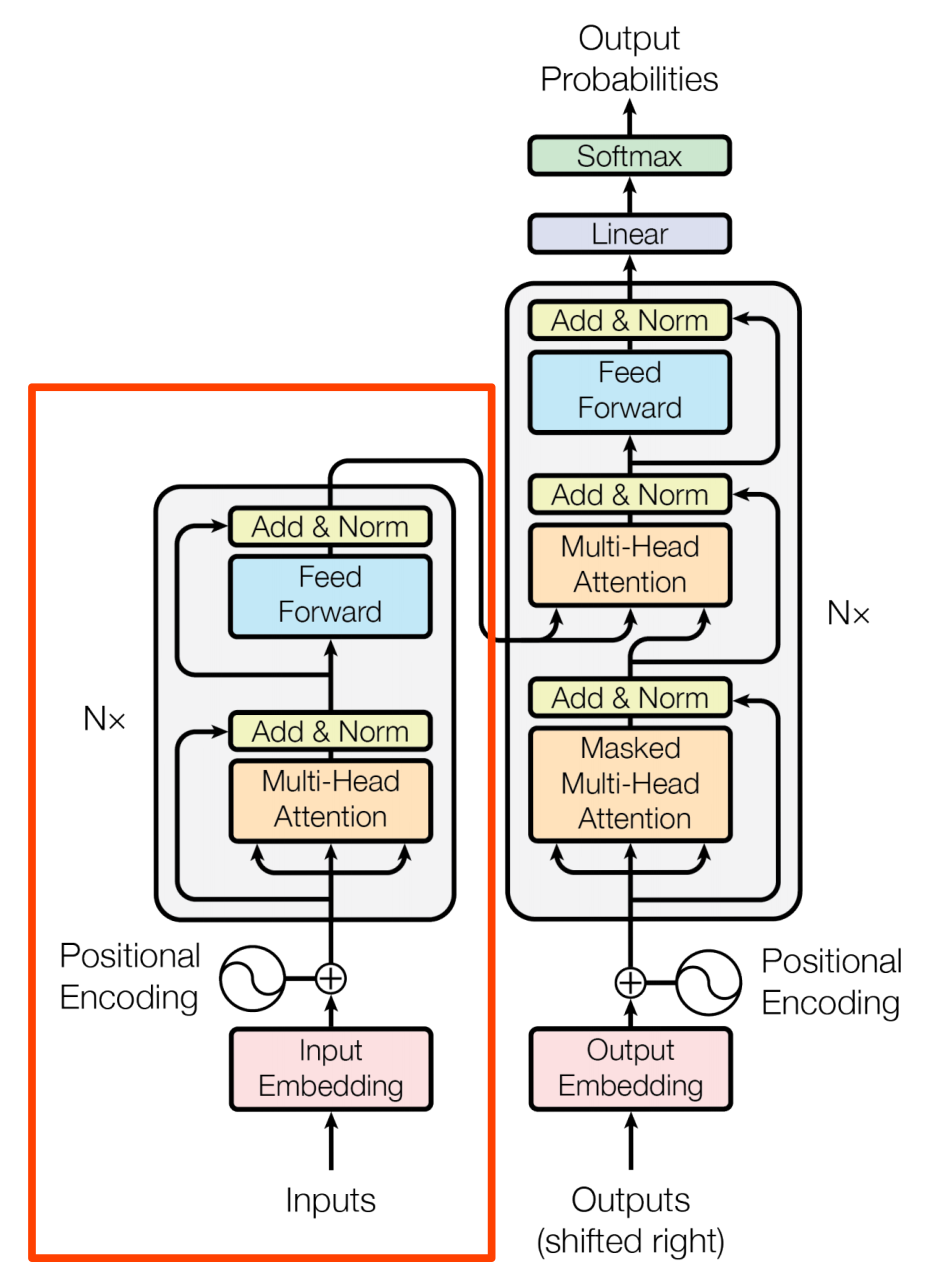
\includegraphics[scale=0.175]{Transformer}
		\caption{Full Transformer architecture}
	\end{figure}
\end{columns}
\end{frame}

\begin{frame}
	\frametitle{Architecture description: Self-Attention}
	
	\begin{columns}
		\column{.6 \textwidth}
		Scaled dot-product attention is a key operation in transformer. It's formula could be written as 
		
		\[ Q = Q W_i^Q \text{ where } W_i^Q \in R^{d_{model} \times d_k} \]
		\[ K = K W_i^K \text{ where } W_i^K \in R^{d_{model} \times d_k} \]
		\[ V = V W_i^V \text{ where } W_i^V \in R^{d_{model} \times d_v}  \]
		\[ Attention(Q, K, V) = softmax \left( \frac{QK^T}{\sqrt{d_k}} \right) V \]
		
		Actually, $Q$, $K$ and $V$ are almost always the same input tensor $X$. But not only one self-attention is being used. We have $h$ heads. After processing sentence of length $L$ through 1 head we get output $O_i \in R^{l \times d_v}$. After concatenation of all heads $conc(O_1, O_2, ..., O_h) \in R^{l \times hd_v}$. Consequently, the last projection matrix is $W_O \in R^{hd_v \times d_{model}}$.
		
		\column{.4 \textwidth}
		\begin{figure}
			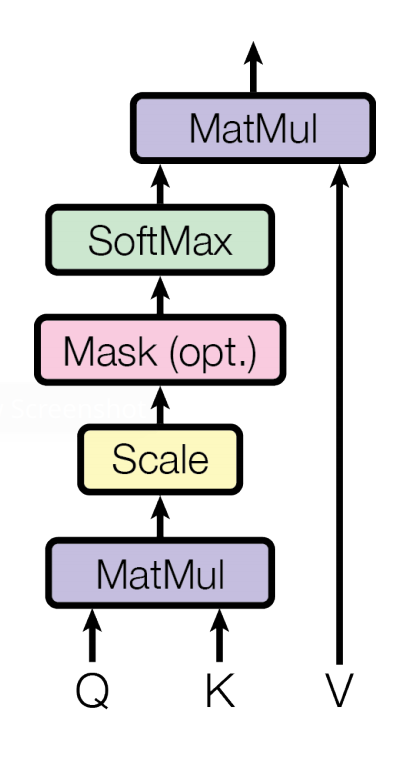
\includegraphics[scale=0.12]{ScaledDotProdAtt}
			\caption{Scaled Dot-Product Attention}
			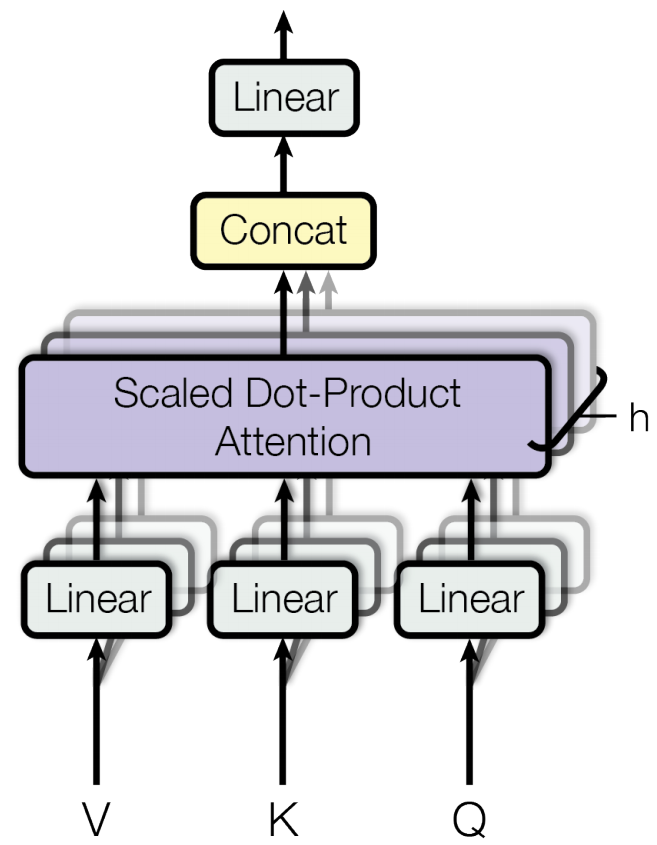
\includegraphics[scale=0.12]{MultiHeadAtt}
			\caption{Multi-Head Attention}
		\end{figure}
	\end{columns}
\end{frame}

\begin{frame}
	\frametitle{Problematic}
	
	Now, when we are familiar with transformer architecture we can discuss it's problems. 
	
	\begin{block}{}
		The main problem of transformer is its' self-attention. It's computation process requires explicit creation, storing and processing of huge matrices. It makes transformer inappropriate to process long sequences. So our further discussion will be about attention complexity reduction.
	\end{block}
	
	For example BERT which is 12 concatenated transformer encoder has a restriction in 512 tokens per sentence. From the next slide we will start to discuss opportunities to improve the original architecture to overcome this issue.
	
\end{frame}

\begin{frame}
	\frametitle{Architecture description: Linformer}
	The main idea of this architecture is that attention matrix is low rank. More detailed:
	
	\begin{block}{Theorem 1}
		For any $Q, K, V \in R^{L \times d_{model}}$ and $W_i^Q, W_i^K, W_i^V \in R^{d_{model} \times d_k}$, for any column vector $w \in R^l$ of matrix $V W_i^V$, there exists a low-rank matrix $\tilde{P} \in R^{l \times l}$ such that
		
		\[ Pr(\| \tilde{P}w^T - Pw^T \| < \epsilon \|Pw^T\|) > 1 - o(1) \]
		
		and $rank(\tilde{P}) = \Theta(\log(n))$	where the context mapping matrix $P$
		
		\[ P = softmax \left( \frac{QW_i^Q (KW_i^K)^T}{\sqrt{d_k}} \right) V W_i^V \]
	\end{block}

	As soon as we have low rank matrix we can use SVD to approximate it. However, it requires computation of SVD on every attention step and it introduces additional complexity so it's not our choice.
	 
\end{frame}

\begin{frame}
	\frametitle{Architecture description: Linformer (continue)}
	
	SVD is the best decomposition but it's too expensive for us. To avoid computing decomposition authors introduce new matrices $E_i, F_i \in R^{C \times L}$ where $L$ is sequence length. So if we choose small $k$ then we can significantly reduce complexion and space.
	
	\begin{block}{Theorem 2}
		For any $Q_i, K_i, V_i \in R^{L \times d_{model}}$ and $W_i^Q, W_i^K, W_i^V \in R^{d_{model} \times d_{k}}$, if $C = \min \{ \Theta (9d_{model} \log(d_{model})/\epsilon^2), 5 \Theta (\log(L)/\epsilon^2) \}$, then there exists matrices $E_i, F_i \in R^{C \times L}$ such that, for any row vector $w$ of matrix $QW_i^Q(KW_i^K)^T / \sqrt{d_{k}}$, we have
		\noindent
		\begin{multline*}
			Pr( \| softmax(wE_i^T)F_i V W_i^V - softmax(w)V W_i^V \| \le \\ \epsilon \|softmax(w)\| \|V W_i^V\| ) > 1 - o(1)
		\end{multline*}
	\end{block}

	So, roughly speaking, we are fitting our decomposition while fitting the neural network.
\end{frame}

\begin{frame}
	\frametitle{Architecture description: Linformer (continue)}
	
	And finally we have the formula
	
	\begin{block}{Final attention formula}
		\[ softmax \left( \frac{QW_i^Q (E_iKW_i^K)^T}{\sqrt{d_k}} \right) F_iVW_i^V \]
	\end{block}
	
\end{frame}

\begin{frame}
	\frametitle{Architecture description: Performer}
	
	The main idea of this algorithm is Attention decomposition. One element of the original attention matrix is
	
	\[ A_{i,j} = \exp\left(\frac{Q_i K_j^T}{\sqrt{d_k}}\right) = \exp \left( \frac{\|Q_i\|_2^2}{2\sqrt{d_k}} \right) \exp \left( -\frac{\|Q_i - K_j\|_2^2}{2\sqrt{d_k}} \right) \exp \left( \frac{\|K_j\|_2^2}{2\sqrt{d_k}} \right) \]
	
	Consequently
	
	\[ A = D_Q B D_K \]
	
	where $D_Q, D_K$ are diagonal and $B \in R^{L \times L}$. The $B$ values look quite similar to Gaussian distribution. And from this authors build generalized attention
	
	\[ A = [g(Q_i^T)K(Q_i^T, K_j^T)h(K_j^T)]_{i,j=1, 2, ..., n} \]
	
	And random feature map $\phi : R^d \rightarrow R^M$ is a probabilistic embedding satisfying
	
	\[ K(x, y) = E [\phi^T(x)\phi(y)] \]  
	
	according to the given $K$, where $M$ is a number of random features.
	
\end{frame}

\begin{frame}
	\frametitle{Architecture description: Performer (continue)}
	
	Further authors noticed that there are exist efficient to compute random feature maps for many kernels used in machine learning, moreover, most of them have quite similar view
	
	\[ \phi(X) = \frac{c}{\sqrt{M}} f^T\left( WX + b \right) \]
	
	For some $W$ and $b$ with i.i.d. components and $f: R \rightarrow R$. Here $c, M$ and $f$ are hyperparameters. Consequently
	
	\[ \hat{Q} = \frac{c}{\sqrt{M}} f^T\left( WQ^T + b \right), \text{    } \hat{K} = \frac{c}{\sqrt{M}} f^T\left( WK^T + b \right) \]
	
	\[ Q' = D_Q \hat{Q}, \text{    } K' = D_K \hat{K} \]
	
	\[ A = E[Q'(K')^T] \]
	
	but we can get unbiased approximation $\hat{A} = Q'(K')^T$
	
\end{frame}

\begin{frame}
	\frametitle{Architecture description: Performer (continue)}
	
	It leads us to the following attention formula
	
	\begin{block}{Final attention formula}
		\[ \hat{Att}(Q, K, V) = diag(Q'((K')^T 1_L))^{-1} Q'((K')^T V) \]
	\end{block}
	
	We don't compute $\hat{A}$ here and it helps us to avoid $L \times L$ complexity in computations and storage. In this parameter $M$ allows to choose a trade-off between computational complexity and approximation quality. 
	
	\begin{block}{Reasonable question: Where are orthogonal random features and how they are used here?}
		It's used in sampling of matrix $W$. The idea is to sample $W$ from class of orthogonal special matrices to reduce matvec complexity and get better approximation result by means of reducing estimation variance. Authors compare two methods: Hadamard ORF and Givens ORF named after the class which $W$ is sampled from. It helps us to reduce matvec complexity to $O(M)$ and $O(M \log (d))$ correspondingly (according to authors). We can use it because attention kernel is Gaussian.
	\end{block} 
	
\end{frame}

\begin{frame}
	\frametitle{Complexity analysis}
	
	Now, when we know about candidates in our comparison, we can analyze their complexities. We will analyze only self-attention parts because FFN part and heading are the same for all architectures. 
	
	\begin{block}{Transformer}
		\begin{itemize}
			\item Space: $O(L^2)$
			\item Time: $O(L^2d_{k})$
		\end{itemize}
	\end{block}

	\begin{block}{Linformer}
		\begin{itemize}
			\item Space: $O(2Cd_{model} + Cd_v + LC)$
			\item Time: $O(2LCd_{model} + Cd_{model}d_v)$
		\end{itemize}
	\end{block}

	\begin{block}{Reformer}
		\begin{itemize}
			\item Space: $O(Ld_v + 2ML + Md_v)$ by using H-ORF to sample $W$.
			\item Time: $O(4LMd_{v} + 2ML)$
		\end{itemize}
	\end{block}
	
\end{frame}

\begin{frame}
	\frametitle{Experiment 1: Inference time}
	\begin{columns}
		\column{.4 \textwidth}
		The graph on the right side shows that linearity of Linformer and Performer is rather confirmed than rejected. We can see that transformer model shows almost invisible nonlinearity and starts growing rather than others. Moreover, vanilla transformer could not deal with sequence of length $2^{10}$ when other two models can deal with such sequences with same parameters.
		
		\column{.6 \textwidth}
		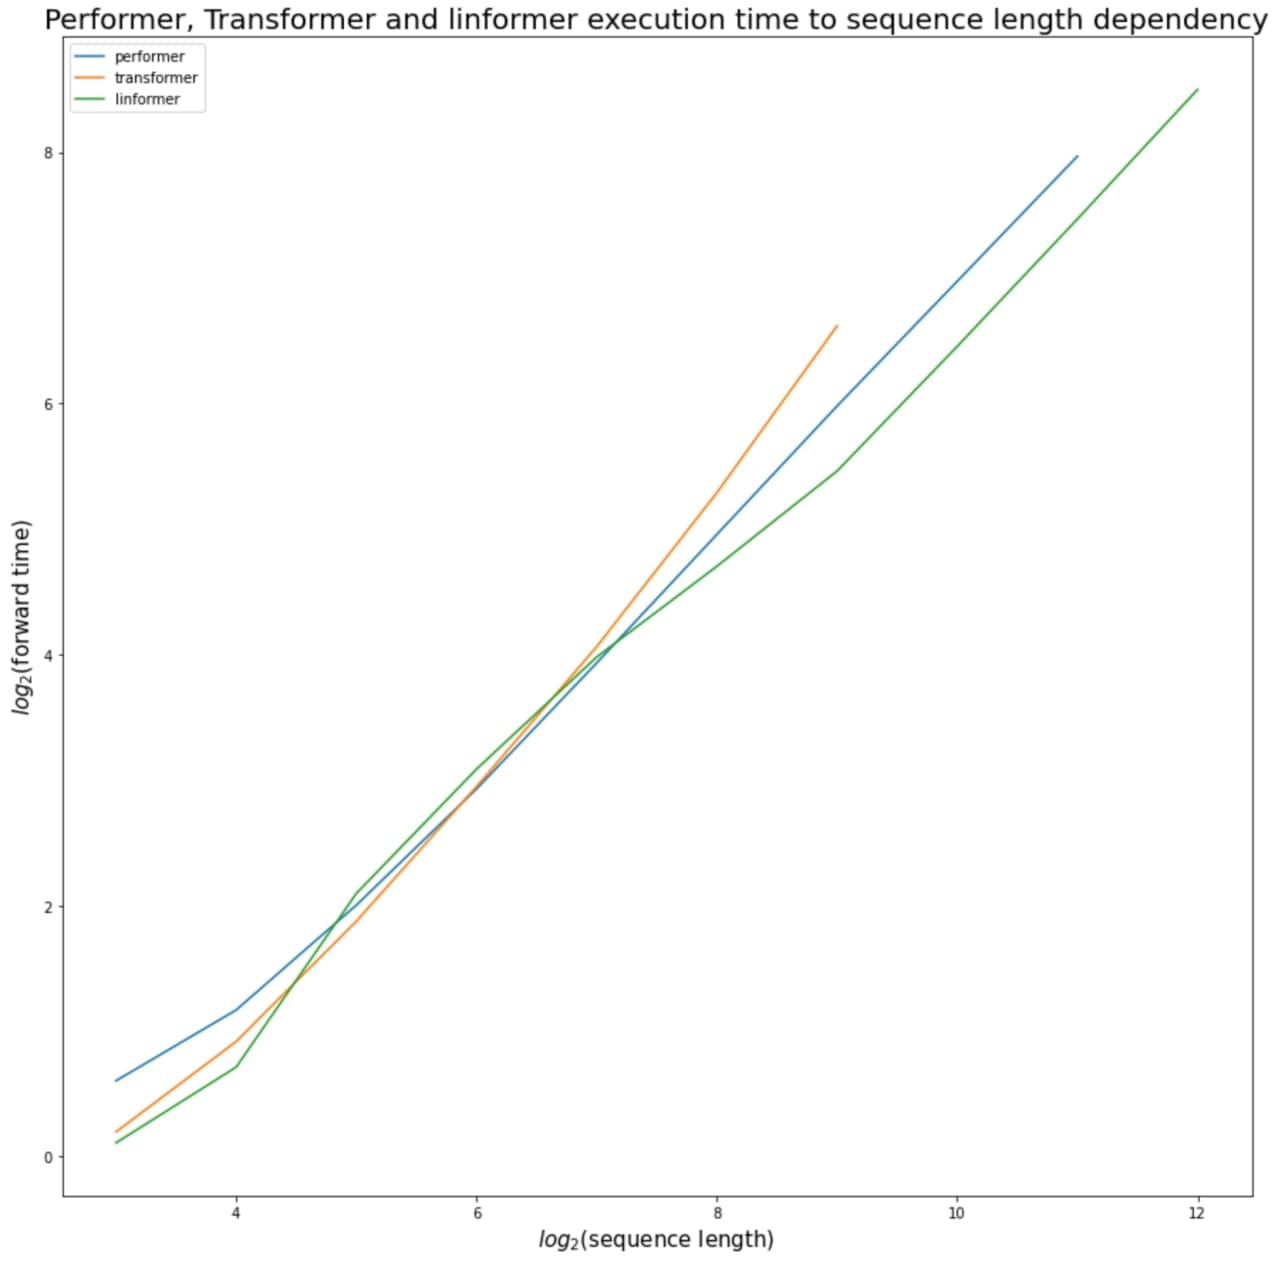
\includegraphics[scale=0.4]{tflfpf_time}
	\end{columns}
	
\end{frame}

\begin{frame}
	\frametitle{Experiment 2: Sequence Length to memory growth}
	
	\begin{columns}
		\column{.6 \textwidth}
		Vanilla transformer parameters doesn't depend on sequence length but the other two models have such parameters. It's interesting to know how sequence length influences the model size.
		
		Both graphs show almost linear memory growth so we can conclude that memory dependency is not a big issue when we talk about these models. 
		
		We also tested our models to compare their quality with original transformer on 3 tasks.
		
		\column{.4 \textwidth}
		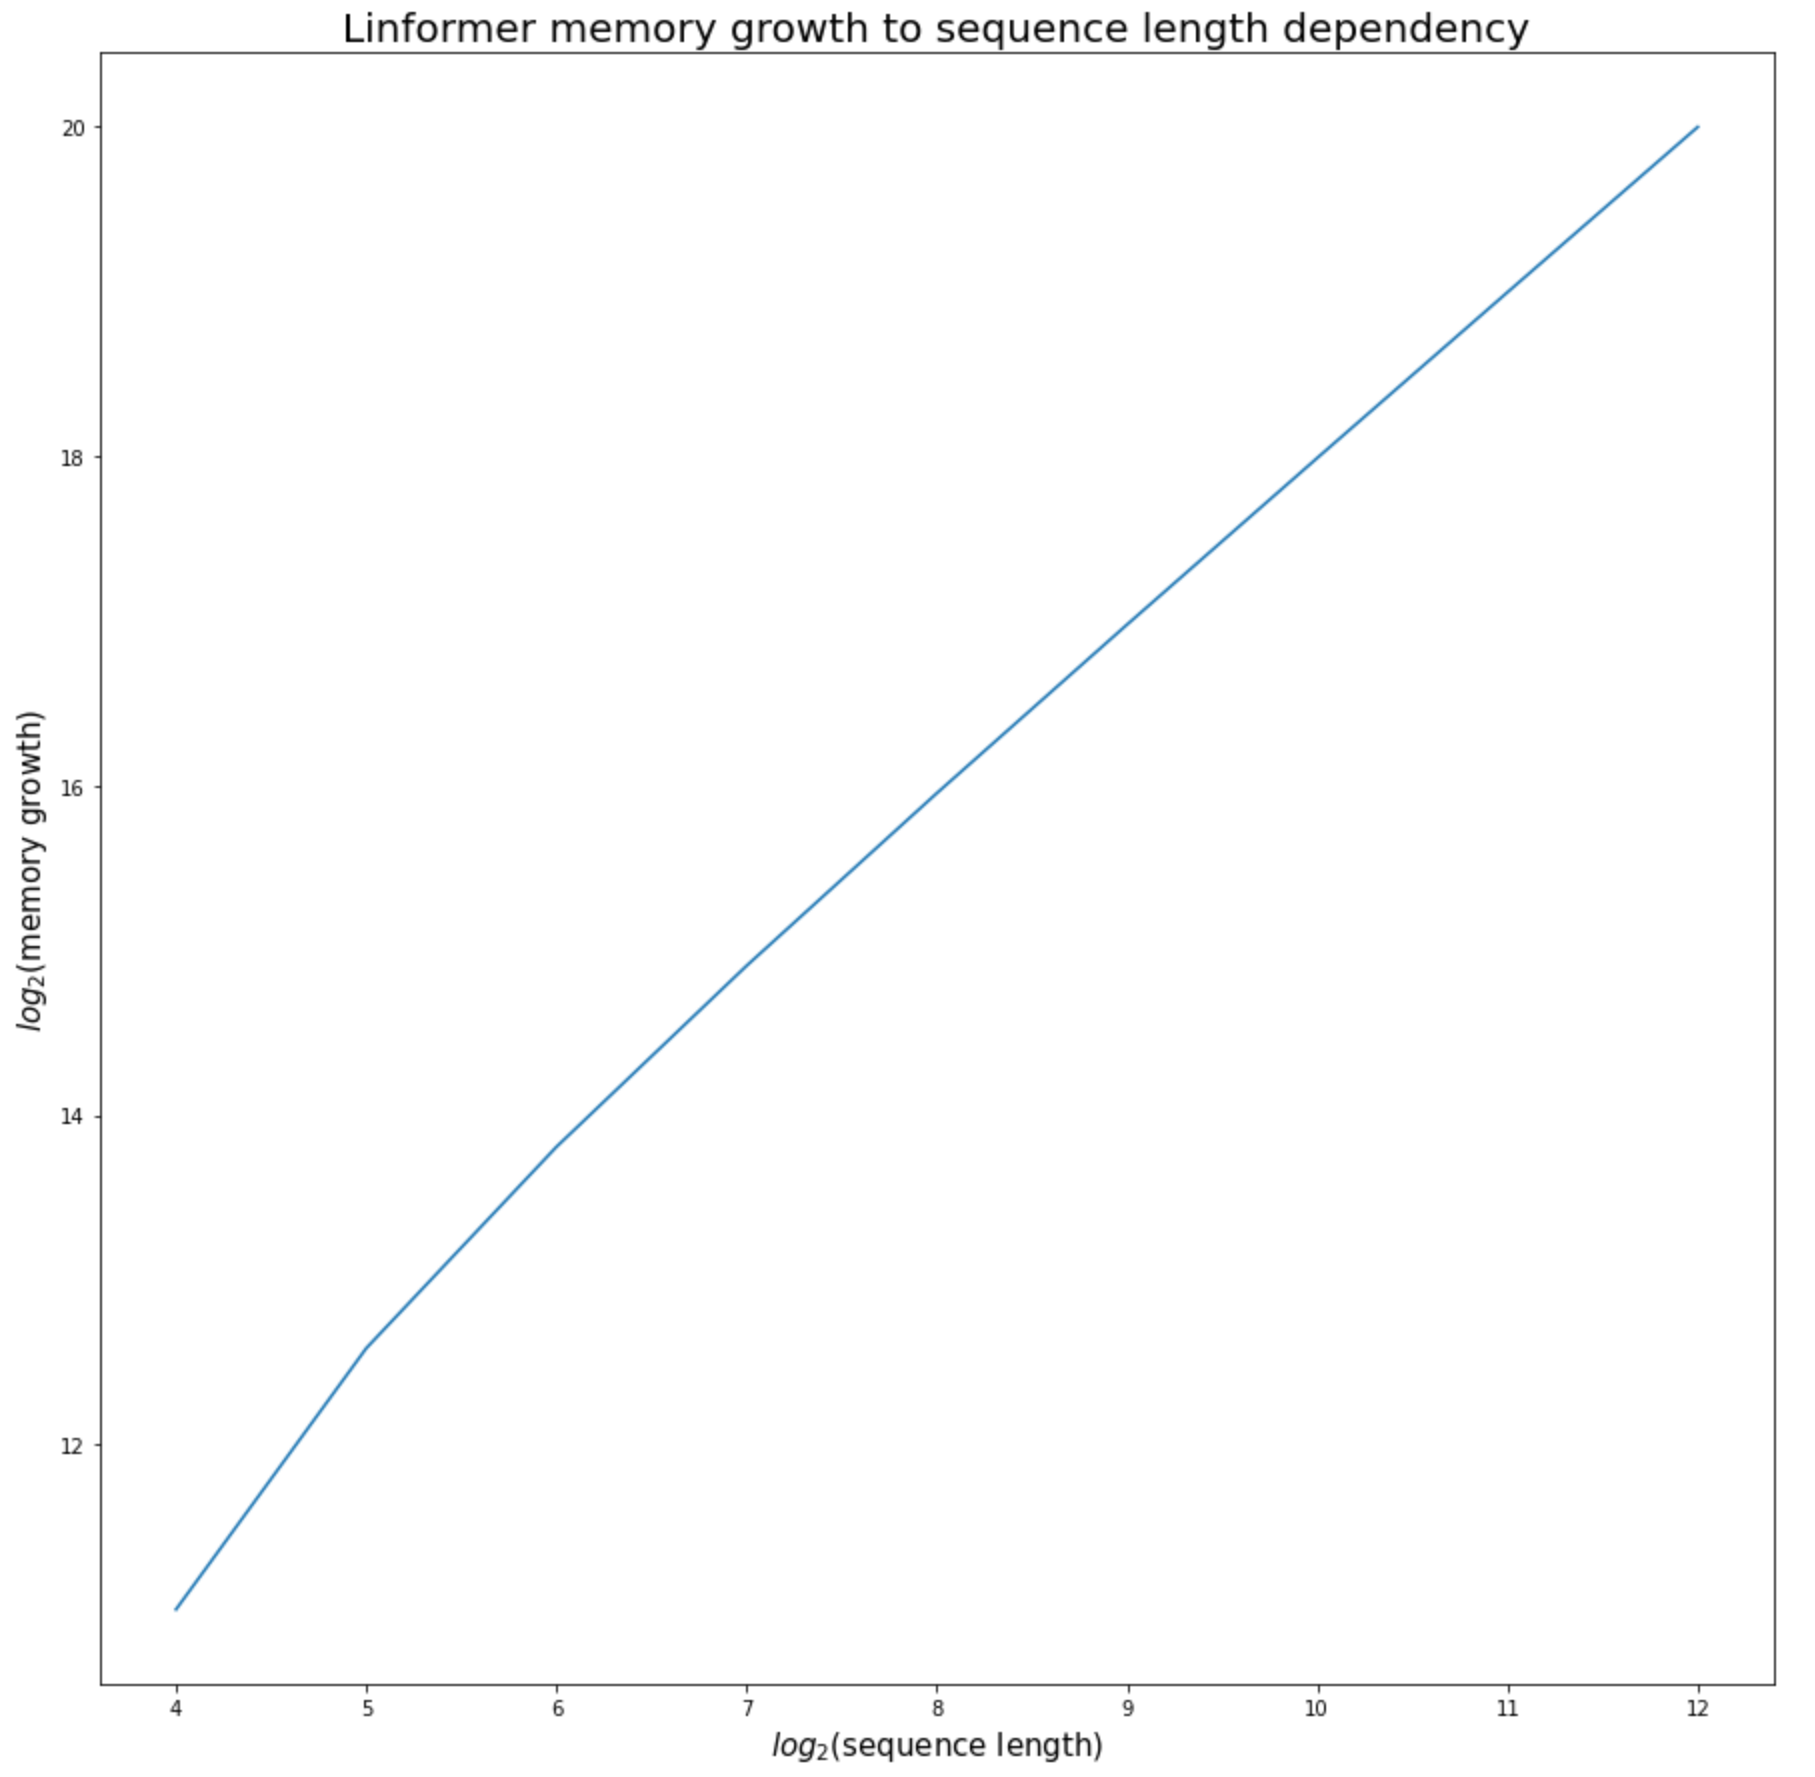
\includegraphics[scale=0.08]{linformer_seq_len_to_memory_growth}
		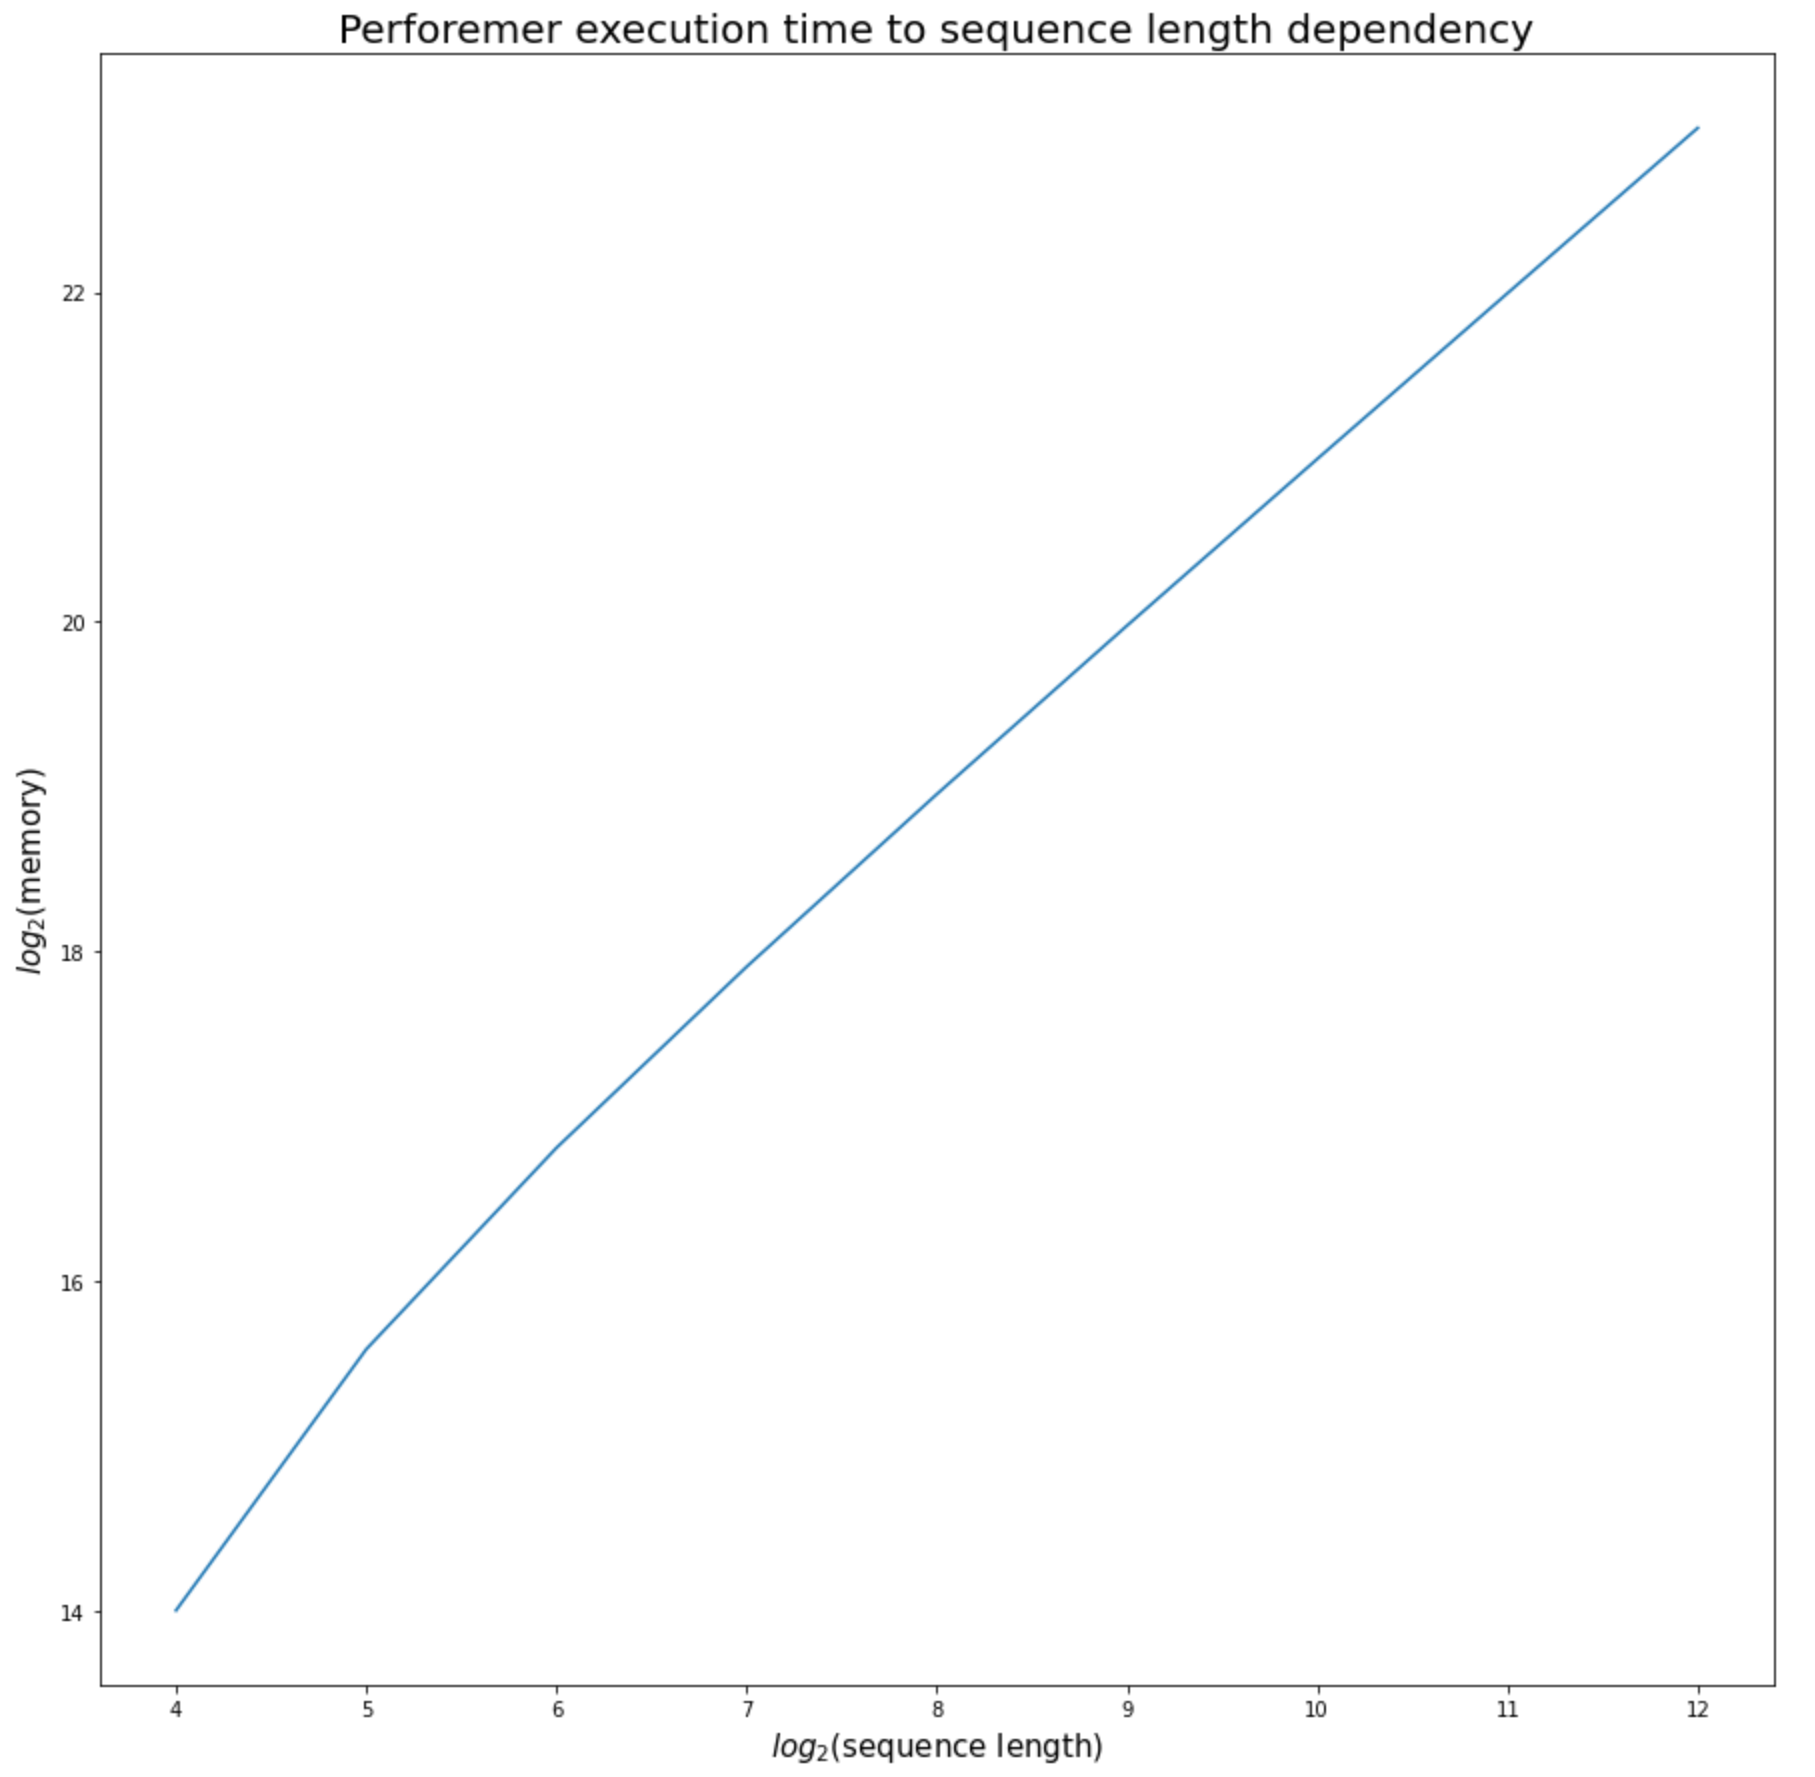
\includegraphics[scale=0.08]{performer_seq_len_to_memory_growth}
	\end{columns}
	
\end{frame}

\begin{frame}
	\frametitle{Experiment 3.1: DistilBERT}
	
	\begin{itemize}
		\item We wanted to try to apply new attention to existing model
		\item We selected DistilBERT because BERT models are very useful but very slow and we wanted to see is it possible to speed them up with such thing as linear attention
		\item We changed casual attention to FAVOR+ (attention used in Performer) and tried to fine-tune model
		\item Perplexity of the resulting model was much higher in comparison with the original model so it means that we didn't succeed
		\item We attribute our fault to the fact that pretrained DistilBERT were received from BERT trained with casual attention and distilled BERT just had not enough degrees of freedom to adopt to new attention.
	\end{itemize}

	We figured out it would be pointless to test our DistilBERT against the original DistilBERT on a downstream task, so we had to find a task which does not require pretraining, and we’ve found it outside the field of NLP.
	
\end{frame}

\begin{frame}
	\frametitle{Experiment 3.2: Modeling point process}
	
	\begin{itemize}
		\item The task was predict next time and next label for a point
		\item We found repository with Transformer code for this task
		\item Firstly we tried to apply casual transformer for this task to get a baseline
		\item We found a bug in authors code and after we removed it we get even better results than described
		\item Then we changed attention to FAVOR+ and tried to fit model until convergence once again with new attention
		\item After the model converged results were even slightly better than baseline
		\item As a conclusion it was success. We prove empirically that Performer is at least compatible to transformer in terms of quality
	\end{itemize}
	
\end{frame}

\begin{frame}
	\frametitle{Conclusion}
	
	\begin{itemize}
		\item We found three transformer architectures with 3 different attention types
		\item We described how they differ and estimated their time and memory complexity
		\item We made some experiments to compare vanilla transformer with it's modifications
		\item We also tested our models on real tasks and obtained results confirming that Performer is not worse than vanilla transformer
	\end{itemize}
	
\end{frame}

\begin{frame}
	
	\huge{Thank you for attention!}
	
\end{frame}

\end{document}